
\chapter*{Introduzione}

Da qualche anno a questa parte sono stati sviluppati e messi in commercio dispositivi per la realtà virtuale, i più famosi sono la Nintendo Wii, il Kinect della Microsoft o l'Oculus Rift sviluppato da Oculus VR. Periferiche come queste sono dette NUI, “natural user interface”\cite{NUI}: essenzialmente sono interfacce per l'interazione con sistemi virtuali e hanno lo scopo di aumentare la sensazione della realtà durante l'utilizzo di applicazioni e simulazioni virtuali, permettendo all'utente di sfruttare più sensi.

La Wii permette, tramite il suo telecomando, di utilizzare indirettamente il corpo umano come dispositivo di input di comandi. Il Kinect utilizza dei sensori a infrarossi e una telecamera per rilevare il corpo umano e registrare direttamente i suoi movimenti, trasformandoli in comandi di input. L'Oculus Rift è un visore che presenta dei sensori che riconoscono l'orientamento della testa, i cui movimenti sono tradotti in rotazioni della telecamera virtuale nell'applicazione, rendendo immersiva la visione, anche grazie alla presenza di due schermi che producono un effetto tridimensionale.

Il progetto trattato in questa tesi mira ad emulare dispositivi di questo genere, utilizzando semplicemente un computer e una webcam. La posizione del volto, rilevata elaborando le immagini acquisite tramite una webcam, determina la prospettiva con cui viene visualizzata una scena tridimensionale, con lo scopo di collegare la telecamera virtuale agli occhi dell'utente. L'obiettivo finale è quello di generare l'illusione della presenza di profondità all'interno dello schermo e di creare, in condizioni ottimali, un effetto tridimensionale senza l'utilizzo di occhiali appositi.

Dato l'utilizzo di dispositivi di qualità medio-bassa, l'effetto generato non è paragonabile a quello che può essere prodotto da sistemi più efficienti e dedicati allo scopo, tuttavia sono stati raggiunti comunque risultati notevoli.

Il progetto è stato sviluppato impiegando i seguenti software e librerie:
\begin{itemize}
\item OpenCV, per il rilevamento del volto.
\item OpenGL, per lo studio di fattibilità e per lo sviluppo di un prototipo.
\item Blender, per la creazione di scene 3D.
\item Ogre3D, per un miglioramento dell'applicazione in termini di grafica ed efficienza.
\end{itemize}

Nel corso di questa tesi si farà un'introduzione sulla realtà virtuale, si parlerà delle tecnologie utilizzate, sarà spiegata la teoria matematica che sta dietro alle trasformazioni applicate, facendo un excursus sulle tecniche adottate dalla maggior parte delle applicazioni grafiche per renderizzare a schermo una scena tridimensionale, ed infine sarà trattato il progetto sviluppato, mostrando anche le problematiche riscontrate e le possibili soluzioni.

\begin{figure}[htbp]
\centering
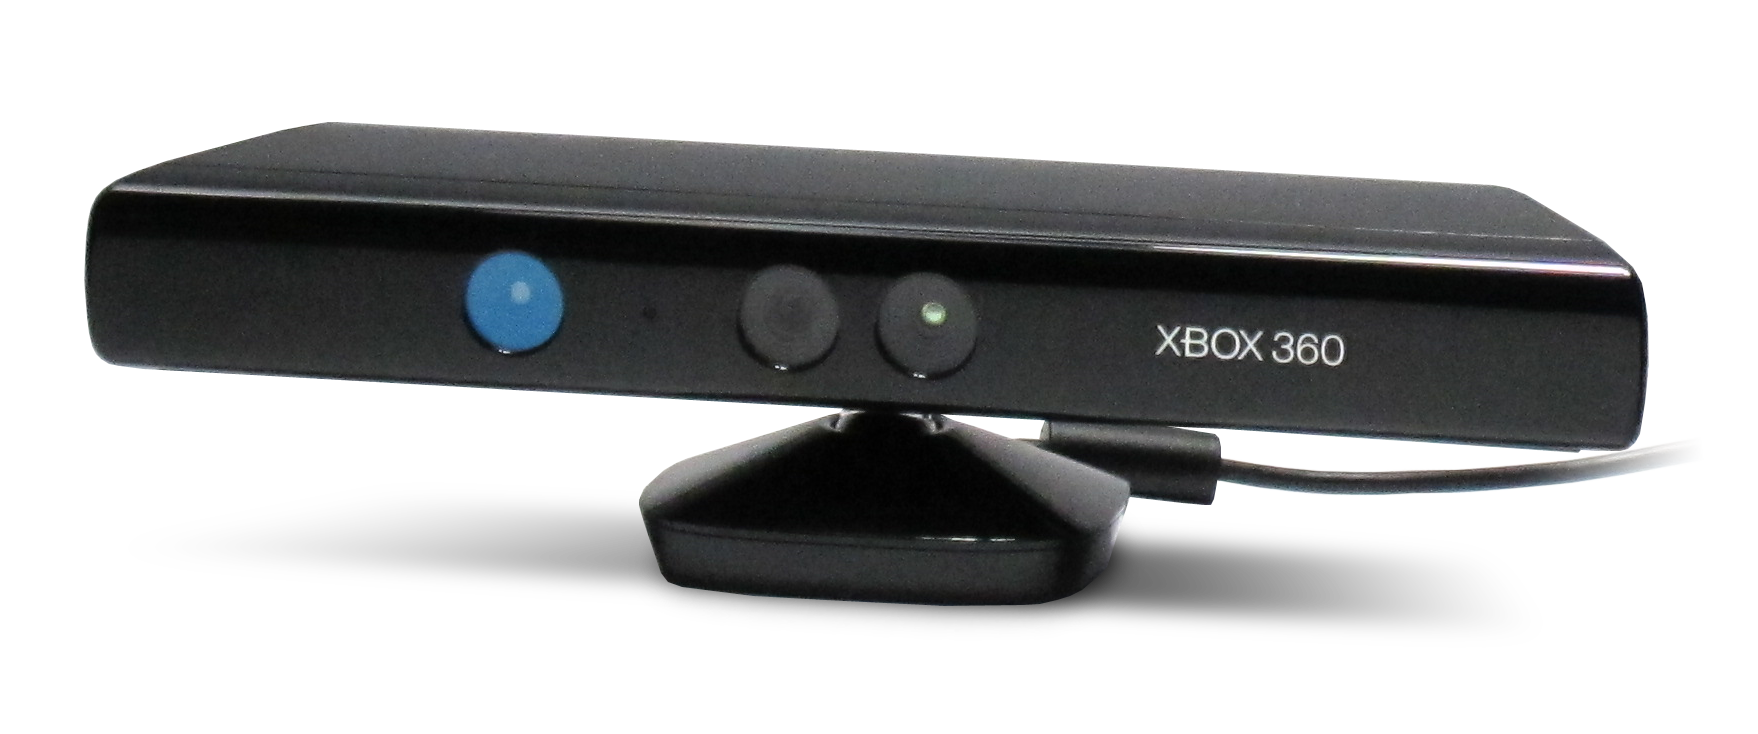
\includegraphics[width=0.4\textwidth]{images/intro/kinect.png}
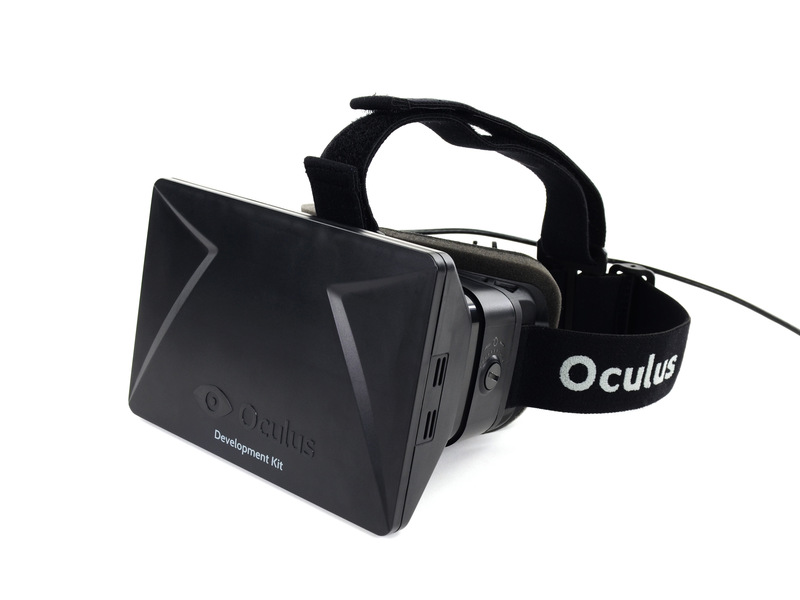
\includegraphics[width=0.4\textwidth]{images/intro/oculus-rift.jpg}
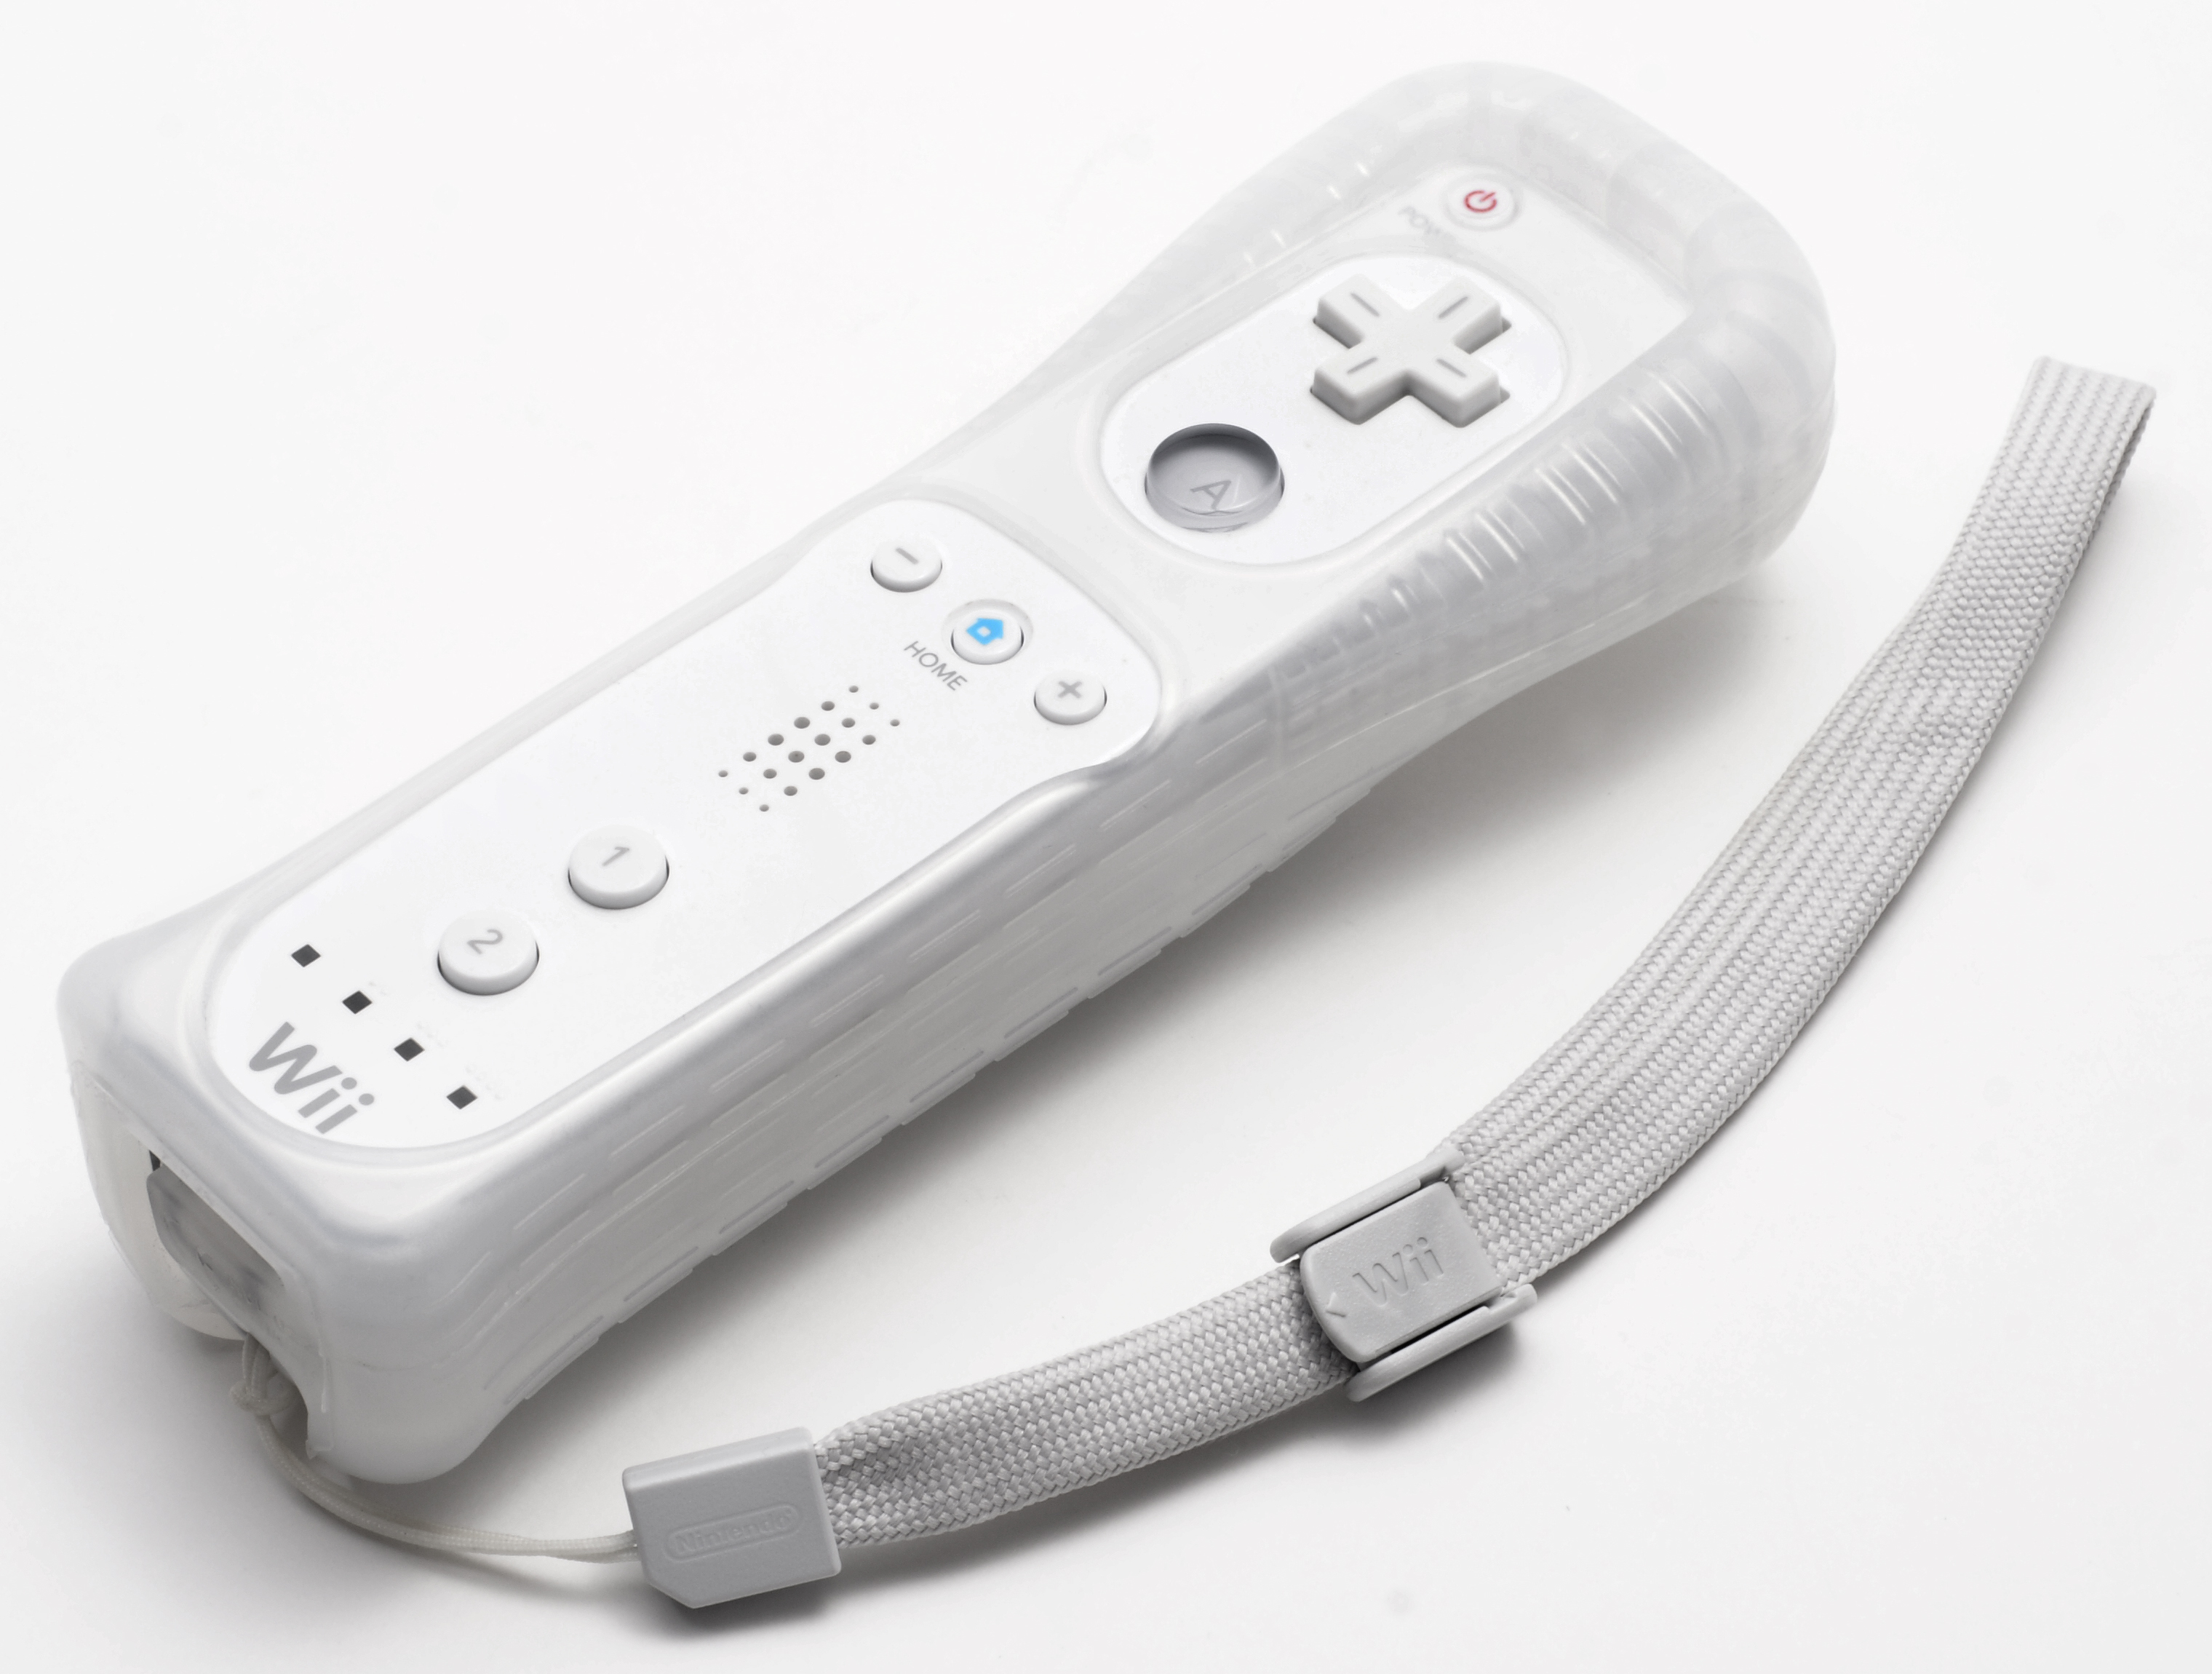
\includegraphics[width=0.4\textwidth]{images/intro/wii.jpg}
\end{figure}
